%% LyX 2.4.3 created this file.  For more info, see https://www.lyx.org/.
%% Do not edit unless you really know what you are doing.
\documentclass[journal,article,submit,pdftex,moreauthors]{Definitions/mdpi}
\usepackage[utf8]{inputenc}
\usepackage{float}
\usepackage{amsmath}
\usepackage{graphicx}

\makeatletter

%%%%%%%%%%%%%%%%%%%%%%%%%%%%%% LyX specific LaTeX commands.

\Title{Constructing artificial features with Grammatical Evolution for the
motor symptoms of Parkinson’s Disease}

\TitleCitation{Constructing artificial features with Grammatical Evolution for the
motor symptoms of Parkinson’s Disease}

\Author{Aimilios Psathas$^{1}$, Ioannis G. Tsoulos$^{2,*}$, Nikolaos Giannakeas$^{3}$,
Alexandros Tzallas$^{4}$ and Vasileios Charilogis$^{5}$}

\AuthorNames{Psathas, A., Tsoulos, I.G., Tzallas, A. \textbackslash\& Charilogis,
V. }

\AuthorNames{Aimilios Psathas, Ioannis G. Tsoulos, Alexandros Tzallas and Vasileios
Charilogis. }

\AuthorCitation{Psathas, A.; Tsoulos, I.G.; Tzallas, A.; Charilogis, V. }


\address{$^{1}$\quad{}Department of Informatics and Telecommunications,
University of Ioannina, Greece;pint00141@uoi.gr\\
$^{2}$\quad{}Department of Informatics and Telecommunications, University
of Ioannina, Greece; itsoulos@uoi.gr\\
$^{3}\quad$Department of Informatics and Telecommunications, University
of Ioannina, Greece; giannakeas@uoi.gr\\
$^{4}\quad$Department of Informatics and Telecommunications, University
of Ioannina, Greece; tzallas@uoi.gr\\
$^{5}\quad$Department of Informatics and Telecommunications, University
of Ioannina, Greece; v.charilog@uoi.gr}


\corres{Correspondence: itsoulos@uoi.gr}


\abstract{This study introduces a set of features designed to capture the motor
symptoms of Parkinson’s Disease (PD) through detailed motion analysis,
with a specific focus on how these symptoms change before and after
medication. The features reflect key aspects of patient movement,
such as tremor intensity, slowness, rigidity, instability, and irregularity
in motion patterns. By quantifying how consistently and smoothly a
patient performs specific tasks, the features provide insight into
motor control quality and neurological function. Crucially, they are
labeled according to the patient's state---before and after receiving
medication---allowing for a clear comparison of treatment effects.
This enables not only objective tracking of symptom severity, but
also evaluation of medication responsiveness. These features address
a fundamental clinical need: moving beyond subjective observation
toward continuous, data-driven monitoring of disease progression and
therapeutic effectiveness in Parkinson’s Disease. In the current work
the impact of feature construction using Grammatical Evolution on
previously mentioned features in evaluated. We compare traditional
neural architectures (MLP with ADAM, MLP with Genetic Algorithm, and
RBF networks) against models trained on artificially constructed features.
The results demonstrate a substantial reduction in classification
error when 2 to 5 constructed features are used, achieving the lowest
error rate (14.33\%) with four generated features (FC4GEN), compared
to 38.65\% for the best baseline model (RBF). These findings highlight
the effectiveness of evolutionary feature construction in enhancing
classification accuracy.}


\keyword{Machine learning; Evolutionary algorithms; Genetic Programming; Grammatical
Evolution}

\DeclareTextSymbolDefault{\textquotedbl}{T1}
%% Because html converters don't know tabularnewline
\providecommand{\tabularnewline}{\\}

%%%%%%%%%%%%%%%%%%%%%%%%%%%%%% Textclass specific LaTeX commands.
\newenvironment{lyxcode}
	{\par\begin{list}{}{
		\setlength{\rightmargin}{\leftmargin}
		\setlength{\listparindent}{0pt}% needed for AMS classes
		\raggedright
		\setlength{\itemsep}{0pt}
		\setlength{\parsep}{0pt}
		\normalfont\ttfamily}%
	 \item[]}
	{\end{list}}

%%%%%%%%%%%%%%%%%%%%%%%%%%%%%% User specified LaTeX commands.
%  LaTeX support: latex@mdpi.com 
%  For support, please attach all files needed for compiling as well as the log file, and specify your operating system, LaTeX version, and LaTeX editor.

%=================================================================
%\documentclass[preprints,article,submit,pdftex,moreauthors]{Definitions/mdpi} 
% For posting an early version of this manuscript as a preprint, you may use "preprints" as the journal. Changing "submit" to "accept" before posting will remove line numbers.

% Below journals will use APA reference format:
% admsci, behavsci, businesses, econometrics, economies, education, ejihpe, famsci, games, humans, ijcs, ijfs, journalmedia, jrfm, languages, psycholint, publications, tourismhosp, youth

% Below journals will use Chicago reference format:
% arts, genealogy, histories, humanities, jintelligence, laws, literature, religions, risks, socsci

%--------------------
% Class Options:
%--------------------
%----------
% journal
%----------
% Choose between the following MDPI journals:
% accountaudit, acoustics, actuators, addictions, adhesives, admsci, adolescents, aerobiology, aerospace, agriculture, agriengineering, agrochemicals, agronomy, ai, air, algorithms, allergies, alloys, amh, analytica, analytics, anatomia, anesthres, animals, antibiotics, antibodies, antioxidants, applbiosci, appliedchem, appliedmath, appliedphys, applmech, applmicrobiol, applnano, applsci, aquacj, architecture, arm, arthropoda, arts, asc, asi, astronomy, atmosphere, atoms, audiolres, automation, axioms, bacteria, batteries, bdcc, behavsci, beverages, biochem, bioengineering, biologics, biology, biomass, biomechanics, biomed, biomedicines, biomedinformatics, biomimetics, biomolecules, biophysica, biosensors, biosphere, biotech, birds, blockchains, bloods, blsf, brainsci, breath, buildings, businesses, cancers, carbon, cardiogenetics, catalysts, cells, ceramics, challenges, chemengineering, chemistry, chemosensors, chemproc, children, chips, cimb, civileng, cleantechnol, climate, clinbioenerg, clinpract, clockssleep, cmd, cmtr, coasts, coatings, colloids, colorants, commodities, complications, compounds, computation, computers, condensedmatter, conservation, constrmater, cosmetics, covid, crops, cryo, cryptography, crystals, csmf, ctn, curroncol, cyber, dairy, data, ddc, dentistry, dermato, dermatopathology, designs, devices, diabetology, diagnostics, dietetics, digital, disabilities, diseases, diversity, dna, drones, dynamics, earth, ebj, ecm, ecologies, econometrics, economies, education, eesp, ejihpe, electricity, electrochem, electronicmat, electronics, encyclopedia, endocrines, energies, eng, engproc, ent, entomology, entropy, environments, epidemiologia, epigenomes, esa, est, famsci, fermentation, fibers, fintech, fire, fishes, fluids, foods, forecasting, forensicsci, forests, fossstud, foundations, fractalfract, fuels, future, futureinternet, futureparasites, futurepharmacol, futurephys, futuretransp, galaxies, games, gases, gastroent, gastrointestdisord, gastronomy, gels, genealogy, genes, geographies, geohazards, geomatics, geometry, geosciences, geotechnics, geriatrics, glacies, grasses, greenhealth, gucdd, hardware, hazardousmatters, healthcare, hearts, hemato, hematolrep, heritage, higheredu, highthroughput, histories, horticulturae, hospitals, humanities, humans, hydrobiology, hydrogen, hydrology, hygiene, idr, iic, ijerph, ijfs, ijgi, ijmd, ijms, ijns, ijpb, ijt, ijtm, ijtpp, ime, immuno, informatics, information, infrastructures, inorganics, insects, instruments, inventions, iot, j, jal, jcdd, jcm, jcp, jcs, jcto, jdad, jdb, jeta, jfb, jfmk, jimaging, jintelligence, jlpea, jmahp, jmmp, jmms, jmp, jmse, jne, jnt, jof, joitmc, joma, jop, jor, journalmedia, jox, jpbi, jpm, jrfm, jsan, jtaer, jvd, jzbg, kidney, kidneydial, kinasesphosphatases, knowledge, labmed, laboratories, land, languages, laws, life, lights, limnolrev, lipidology, liquids, literature, livers, logics, logistics, lubricants, lymphatics, machines, macromol, magnetism, magnetochemistry, make, marinedrugs, materials, materproc, mathematics, mca, measurements, medicina, medicines, medsci, membranes, merits, metabolites, metals, meteorology, methane, metrics, metrology, micro, microarrays, microbiolres, microelectronics, micromachines, microorganisms, microplastics, microwave, minerals, mining, mmphys, modelling, molbank, molecules, mps, msf, mti, multimedia, muscles, nanoenergyadv, nanomanufacturing, nanomaterials, ncrna, ndt, network, neuroglia, neurolint, neurosci, nitrogen, notspecified, nursrep, nutraceuticals, nutrients, obesities, oceans, ohbm, onco, oncopathology, optics, oral, organics, organoids, osteology, oxygen, parasites, parasitologia, particles, pathogens, pathophysiology, pediatrrep, pets, pharmaceuticals, pharmaceutics, pharmacoepidemiology, pharmacy, philosophies, photochem, photonics, phycology, physchem, physics, physiologia, plants, plasma, platforms, pollutants, polymers, polysaccharides, populations, poultry, powders, preprints, proceedings, processes, prosthesis, proteomes, psf, psych, psychiatryint, psychoactives, psycholint, publications, purification, quantumrep, quaternary, qubs, radiation, reactions, realestate, receptors, recycling, regeneration, religions, remotesensing, reports, reprodmed, resources, rheumato, risks, robotics, rsee, ruminants, safety, sci, scipharm, sclerosis, seeds, sensors, separations, sexes, signals, sinusitis, siuj, skins, smartcities, sna, societies, socsci, software, soilsystems, solar, solids, spectroscj, sports, standards, stats, std, stresses, surfaces, surgeries, suschem, sustainability, symmetry, synbio, systems, tae, targets, taxonomy, technologies, telecom, test, textiles, thalassrep, therapeutics, thermo, timespace, tomography, tourismhosp, toxics, toxins, transplantology, transportation, traumacare, traumas, tropicalmed, universe, urbansci, uro, vaccines, vehicles, venereology, vetsci, vibration, virtualworlds, viruses, vision, waste, water, wem, wevj, wild, wind, women, world, youth, zoonoticdis

%---------
% article
%---------
% The default type of manuscript is "article", but can be replaced by: 
% abstract, addendum, article, book, bookreview, briefreport, casereport, comment, commentary, communication, conferenceproceedings, correction, conferencereport, entry, expressionofconcern, extendedabstract, datadescriptor, editorial, essay, erratum, hypothesis, interestingimage, obituary, opinion, projectreport, reply, retraction, review, perspective, protocol, shortnote, studyprotocol, systematicreview, supfile, technicalnote, viewpoint, guidelines, registeredreport, tutorial
% supfile = supplementary materials

%----------
% submit
%----------
% The class option "submit" will be changed to "accept" by the Editorial Office when the paper is accepted. This will only make changes to the frontpage (e.g., the logo of the journal will get visible), the headings, and the copyright information. Also, line numbering will be removed. Journal info and pagination for accepted papers will also be assigned by the Editorial Office.

%------------------
% moreauthors
%------------------
% If there is only one author the class option oneauthor should be used. Otherwise use the class option moreauthors.

%---------
% pdftex
%---------
% The option pdftex is for use with pdfLaTeX. If eps figures are used, remove the option pdftex and use LaTeX and dvi2pdf.

%=================================================================
% MDPI internal commands - do not modify
\firstpage{1} 
\setcounter{page}{\@firstpage}
\pubvolume{1}
\issuenum{1}
\articlenumber{0}
\pubyear{2025}
\copyrightyear{2025}
%\externaleditor{Firstname Lastname} % More than 1 editor, please add `` and '' before the last editor name
\datereceived{}
\daterevised{ } % Comment out if no revised date
\dateaccepted{}
\datepublished{}
%\datecorrected{} % For corrected papers include a "Corrected: XXX" date in the original paper.
%\dateretracted{} % For retracted papers include a "RETRACTED: XXX" date in the original paper.
\hreflink{https://doi.org/} % If needed use \linebreak
%\doinum{}
%\pdfoutput=1 % Uncommented for upload to arXiv.org
%\CorrStatement{yes}  % For updates
%\longauthorlist{yes} % For many authors that exceed the left citation part

%=================================================================
% Add packages and commands here. The following packages are loaded in our class file: fontenc, inputenc, calc, indentfirst, fancyhdr, graphicx, epstopdf, lastpage, ifthen, lineno, float, amsmath, setspace, enumitem, mathpazo, booktabs, titlesec, etoolbox, tabto, xcolor, soul, multirow, microtype, tikz, totcount, changepage, attrib, upgreek, cleveref, amsthm, hyphenat, natbib, hyperref, footmisc, url, geometry, newfloat, caption

%=================================================================
%% Please use the following mathematics environments: Theorem, Lemma, Corollary, Proposition, Characterization, Property, Problem, Example, ExamplesandDefinitions, Hypothesis, Remark, Definition, Notation, Assumption
%% For proofs, please use the proof environment (the amsthm package is loaded by the MDPI class).

%=================================================================
% The fields PACS, MSC, and JEL may be left empty or commented out if not applicable
%\PACS{J0101}
%\MSC{}
%\JEL{}

%%%%%%%%%%%%%%%%%%%%%%%%%%%%%%%%%%%%%%%%%%
% Only for the journal Diversity
%\LSID{\url{http://}}

%%%%%%%%%%%%%%%%%%%%%%%%%%%%%%%%%%%%%%%%%%
% Only for the journal Applied Sciences:
%\featuredapplication{Authors are encouraged to provide a concise description of the specific application or a potential application of the work. This section is not mandatory.}
%%%%%%%%%%%%%%%%%%%%%%%%%%%%%%%%%%%%%%%%%%

%%%%%%%%%%%%%%%%%%%%%%%%%%%%%%%%%%%%%%%%%%
% Only for the journal Data:
%\dataset{DOI number or link to the deposited data set in cases where the data set is published or set to be published separately. If the data set is submitted and will be published as a supplement to this paper in the journal Data, this field will be filled by the editors of the journal. In this case, please make sure to submit the data set as a supplement when entering your manuscript into our manuscript editorial system.}

%\datasetlicense{license under which the data set is made available (CC0, CC-BY, CC-BY-SA, CC-BY-NC, etc.)}

%%%%%%%%%%%%%%%%%%%%%%%%%%%%%%%%%%%%%%%%%%
% Only for the journal Toxins
%\keycontribution{The breakthroughs or highlights of the manuscript. Authors can write one or two sentences to describe the most important part of the paper.}

%%%%%%%%%%%%%%%%%%%%%%%%%%%%%%%%%%%%%%%%%%
% Only for the journal Encyclopedia
%\encyclopediadef{Instead of the abstract}
%\entrylink{The Link to this entry published on the encyclopedia platform.}
%%%%%%%%%%%%%%%%%%%%%%%%%%%%%%%%%%%%%%%%%%

%%%%%%%%%%%%%%%%%%%%%%%%%%%%%%%%%%%%%%%%%%
% Only for the journal Advances in Respiratory Medicine, Smart Cities and Sensors
%\addhighlights{yes}
%\renewcommand{\addhighlights}{%

%\noindent This is an obligatory section in “Advances in Respiratory Medicine”, whose goal is to increase the discoverability and readability of the article via search engines and other scholars. Highlights should not be a copy of the abstract, but a simple text allowing the reader to quickly and simplified find out what the article is about and what can be cited from it. Each of these parts should be devoted up to 2~bullet points.\vspace{3pt}\\
%\textbf{What are the main findings?}
% \begin{itemize}[labelsep=2.5mm,topsep=-3pt]
% \item First bullet.
% \item Second bullet.
% \end{itemize}\vspace{3pt}
%\textbf{What is the implication of the main finding?}
% \begin{itemize}[labelsep=2.5mm,topsep=-3pt]
% \item First bullet.
% \item Second bullet.
% \end{itemize}
%}
%%%%%%%%%%%%%%%%%%%%%%%%%%%%%%%%%%%%%%%%%%

\makeatother

\begin{document}
\maketitle

\section{Introduction}

\section{Materials and Methods}

\subsection{Preliminaries }

\subsection{\label{subsec:Preliminaries}}

Grammatical Evolution procedure can be considered as a genetic algorithm,
where the chromosomes are sets of randomly chosen integers. These
integers represent production rules of the provided BNF grammar \citep{bnf1}.
BNF grammars are usually expressed as sets having the form \textbf{$G=\left(N,T,S,P\right)$},
where
\begin{itemize}
\item The set\textbf{ $N$ }contains the non-terminal symbols of the grammar.
\item The set \textbf{$T$ }includes the terminal symbols of the grammar.\textbf{ }
\item $S$ denotes the start symbol of the grammar, with $S\in N$.
\item \textbf{$P$ }is the set of production rules of the grammar. 
\end{itemize}
The Grammatical Evolution procedure utilizes an extended version of
the initial BNF grammar by adding enumeration in the the production
rules. As an example of an extended BNF grammar consider the grammar
shown in\textbf{ }Figure \ref{fig:BNF-grammar-of}.\textbf{ }The notation
\textless{} \textgreater{} is used to enclose the non - terminal symbols
of the grammar. The value $d$ denotes the dimension of the input
data. The Grammatical Evolution procedure starts from the start symbol
of the program and gradually it creates valid programs in the underlying
language, using the production rules of the grammar. The general scheme
of the production procedure has as follows:
\begin{itemize}
\item \textbf{Get} the next element V from the chromosome that is under
processing.
\item \textbf{Select} the next rule using the equation Rule = V mod NR.
The symbol NR denotes the number of production rules for the under
processing non -- terminal symbol. 
\end{itemize}
A full working example of the production procedure is the chromosome
\[
x=\left[9,8,6,4,16,10,17,23,8,14\right]
\]
 with $d=3$. After a series of steps, the function $f(x)=x_{2}+\cos\left(x_{3}\right)$
is produced for the grammar of Figure \ref{fig:BNF-grammar-of}. The
production steps are shown in Table \ref{tab:table_with_steps}. 

\begin{figure}
\caption{An example of an extended BNF grammar.\label{fig:BNF-grammar-of}}

\begin{lyxcode}
S::=\textless expr\textgreater ~~~(0)~

\textless expr\textgreater ~::=~~(\textless expr\textgreater ~\textless op\textgreater ~\textless expr\textgreater )~~(0)~~~~~~~~~~~~~

~~~~~~~~~~~\textbar ~\textless func\textgreater ~(~\textless expr\textgreater ~)~~~~(1)~~~~~~~~~~~~~

~~~~~~~~~~~\textbar\textless terminal\textgreater ~~~~~~~~~~~~(2)~

\textless op\textgreater ~::=~~~~~+~~~~~~(0)~~~~~~~~~~~~~

~~~~~~~~~~~\textbar ~-~~~~~~(1)~~~~~~~~~~~~~

~~~~~~~~~~~\textbar ~{*}~~~~~~(2)~~~~~~~~~~~~~

~~~~~~~~~~~\textbar ~/~~~~~~(3)

\textless func\textgreater ~::=~~~sin~~(0)~~~~~~~~~~~~~

~~~~~~~~~~~\textbar ~cos~~(1)~~~~~~~~~~~~~

~~~~~~~~~~~\textbar exp~~~(2)~~~~~~~~~~~~~

~~~~~~~~~~~\textbar log~~~(3)

\textless terminal\textgreater ::=\textless xlist\textgreater ~~~~~~~~~~~~~~~~(0)~~~~~~~~~~~~~~~~~~~~~~

~~~~~~~~~~~\textbar\textless dlist\textgreater .\textless dlist\textgreater ~(1)

\textless xlist\textgreater ::=x1~~~~(0)~~~~~~~~~~~~~~

~~~~~~~~~~~\textbar ~x2~(1)~~~~~~~~~~~~~~

~~~~~~~~~~~………~~~~~~~~~~~~~

~~~~~~~~~~~\textbar ~xd~(d-1)

\textless dlist\textgreater ::=\textless digit\textgreater ~~~~~~~~~~~~~~~~~~(0)~~~~~~~~~~~~~~~~~

~~~~~~~~~~~\textbar ~\textless digit\textgreater\textless digit\textgreater ~~~~~~~~~~~~(1)

~~~~~~~~~~~\textbar ~\textless digit\textgreater\textless digit\textgreater\textless digit\textgreater ~~~~~(2)

\textless digit\textgreater ~~::=~0~(0)~~~~~~~~~~~~~

~~~~~~~~~~~\textbar ~1~(1)~~~~~~~~~~~~~

~~~~~~~~~~~\textbar ~2~(2)~~~~~~~~~~~~~

~~~~~~~~~~~\textbar ~3~(3)~~~~~~~~~~~~~

~~~~~~~~~~~\textbar ~4~(4)~~~~~~~~~~~~~

~~~~~~~~~~~\textbar ~5~(5)~~~~~~~~~~~~~

~~~~~~~~~~~\textbar ~6~(6)~~~~~~~~~~~~~

~~~~~~~~~~~\textbar ~7~(7)~~~~~~~~~~~~~

~~~~~~~~~~~\textbar ~8~(8)~~~~~~~~~~~~~

~~~~~~~~~~~\textbar ~9~(9)
\end{lyxcode}
\end{figure}
\begin{table}
\caption{A series of production steps for the example chromosome. \label{tab:table_with_steps}}

\centering{}%
\begin{tabular}{|c|c|c|}
\hline 
String & Chromosome & Operation\tabularnewline
\hline 
\hline 
\textless expr\textgreater{} & 9,8,6,4,16,10,17,23,8,14 & $9\mod 3=0$\tabularnewline
\hline 
(\textless expr\textgreater\textless op\textgreater\textless expr\textgreater ) & 8,6,4,16,10,17,23,8,14 & $8\mod 3=2$\tabularnewline
\hline 
(\textless terminal\textgreater\textless op\textgreater\textless expr\textgreater ) & 6,4,16,10,17,23,8,14 & $6\mod 2=0$\tabularnewline
\hline 
(\textless xlist\textgreater\textless op\textgreater\textless expr\textgreater ) & 4,16,10,17,23,8,14 & $4\mod 3=1$\tabularnewline
\hline 
(x2\textless op\textgreater\textless expr\textgreater ) & 16,10,17,23,8,14 & $16\mod 4=0$\tabularnewline
\hline 
(x2+\textless expr\textgreater ) & 10,17,23,8,14 & $10\mod 3=1$\tabularnewline
\hline 
(x2+\textless func\textgreater (\textless expr\textgreater )) & 17,23,8,14 & $17\mod 4=1$\tabularnewline
\hline 
(x2+cos(\textless expr\textgreater )) & 23,8,14 & $23\mod 2=2$\tabularnewline
\hline 
(x2+cos(\textless terminal\textgreater )) & 8,14 & $8\mod 2=0$\tabularnewline
\hline 
(x2+cos(\textless xlist\textgreater )) & 14 & $14\mod 3=2$\tabularnewline
\hline 
(x2+cos(x3)) &  & \tabularnewline
\hline 
\end{tabular}
\end{table}


\subsection{The feature construction method}

The technique of feature construction produces artificial features
for classification or regression problems as non - linear transformations
of the original ones. The new features are evaluated using a machine
learning technique, such as artificial neural networks \citep{nn1,nn2}
or a Radial Basis Function (RBF) networks \citep{rbf1,rbf2}. This
method was presented initially in \citep{fc1}. Also, this method
was used in many areas, such as Spam Identification \citep{fc2},
Fetal heart classification \citep{fc3},\textbf{ }signal processing
\citep{fc4,fc5} etc. The process has the following steps:
\begin{enumerate}
\item \textbf{Initialization} step. \textbf{}

\begin{enumerate}
\item \textbf{Obtain }the train data for the current problem. The train
data have $M$ pairs\textbf{ $\left(x_{i},t_{i}\right),\ i=1..M$}.
The dimension of each vector $x_{i}$ is\textbf{ $d$.} The values
$t_{i}$ are the expected outputs for each pattern.
\item \textbf{Define }the parameters of the genetic algorithm: \textbf{$N_{g}$}
stands for the the number of allowed generations, \textbf{$N_{c}$
}represents the number chromosomes,\textbf{ $p_{s}$ }defines the
selection rate and \textbf{$p_{m}$} the mutation rate.
\item \textbf{Set} as $N_{f}$ the number of features that will construct
the Grammatical Evolution procedure.
\item \textbf{Initialize} the chromosomes in the population. Each chromosome
is considered as a set of randomly chosen positive integers.
\item \textbf{Set} $k=1$, as the generation counter.
\end{enumerate}
\item \textbf{Genetic step}

\begin{enumerate}
\item \textbf{For $i=1,\ldots,N_{c}$ do}

\begin{enumerate}
\item \textbf{Produce} using the Grammatical Evolution procedure a set of
$N_{f}$ artificial features for the corresponding chromosome $g_{i}$.
These features are produced using the grammar of Figure \ref{fig:BNF-grammar-of}.
\item \textbf{Transform} the original dataset using the previously constructed
features. The new training set is denoted as $\left(x_{g_{i},j},t_{j}\right),\ j=1,..M$
\item \textbf{Train }a machine learning model denoted as $C$ using the
new training set. The fitness $f_{i}$ for the corresponding chromosome
is defined as:
\begin{equation}
f_{i}=\sum_{j=1}^{M}\left(C\left(x_{g_{i},j}\right)-t_{j}\right)^{2}
\end{equation}
In the proposed method the RBF network is used as the machine learning
model, since the time required for its training is significantly lower
than other models, such as neural networks.
\item \textbf{Perform} the selection procedure. During this procedure the
chromosomes are firstly sorted according to their fitness values and
the best\textbf{ $\left(1-p_{s}\right)\times N_{C}$} of them are
copied intact to the next generation.\textbf{ }The rest of the chromosomes
will be substituted by new chromosomes produced during the procedures
of crossover and mutation. 
\item \textbf{Perform} the crossover procedure. During this procedure $p_{s}\times N_{c}$
new chromosomes are produced. For every pair of $\left(\tilde{z},\tilde{w}\right)$
of new chromosomes, two two distinct chromosomes $\left(z,w\right)$
are selected from the current population. The selection is performed
using the tournament selection. The new chromosomes are produced from
the old ones using the one - point crossover procedure, which is graphically
outlined in Figure \ref{fig:One-point-crossover}. 
\item \textbf{(OK)Perform} the mutation procedure: for each each element
of each chromosome, a random number $r\in\left[0,1\right]$ is selected.
The underlying element is altered randomly when $r\le p_{m}$. 
\end{enumerate}
\item \textbf{EndFor}
\end{enumerate}
\item \textbf{Set} $k=k+1$
\item \textbf{If} $k\le N_{G}$ goto \textbf{Genetic} Step, else terminate
the process and obtain the best chromosome $g^{*}$ with the lowest
fitness value.
\item \textbf{Transform} the corresponding test set, using the $N_{f}$
features obtained for chromosome \textbf{$g^{*}$.}
\item \textbf{Apply} a machine learning model to the constructed test set
and report the associated test error.\textbf{.}

\end{enumerate}
\begin{figure}[H]
\begin{centering}
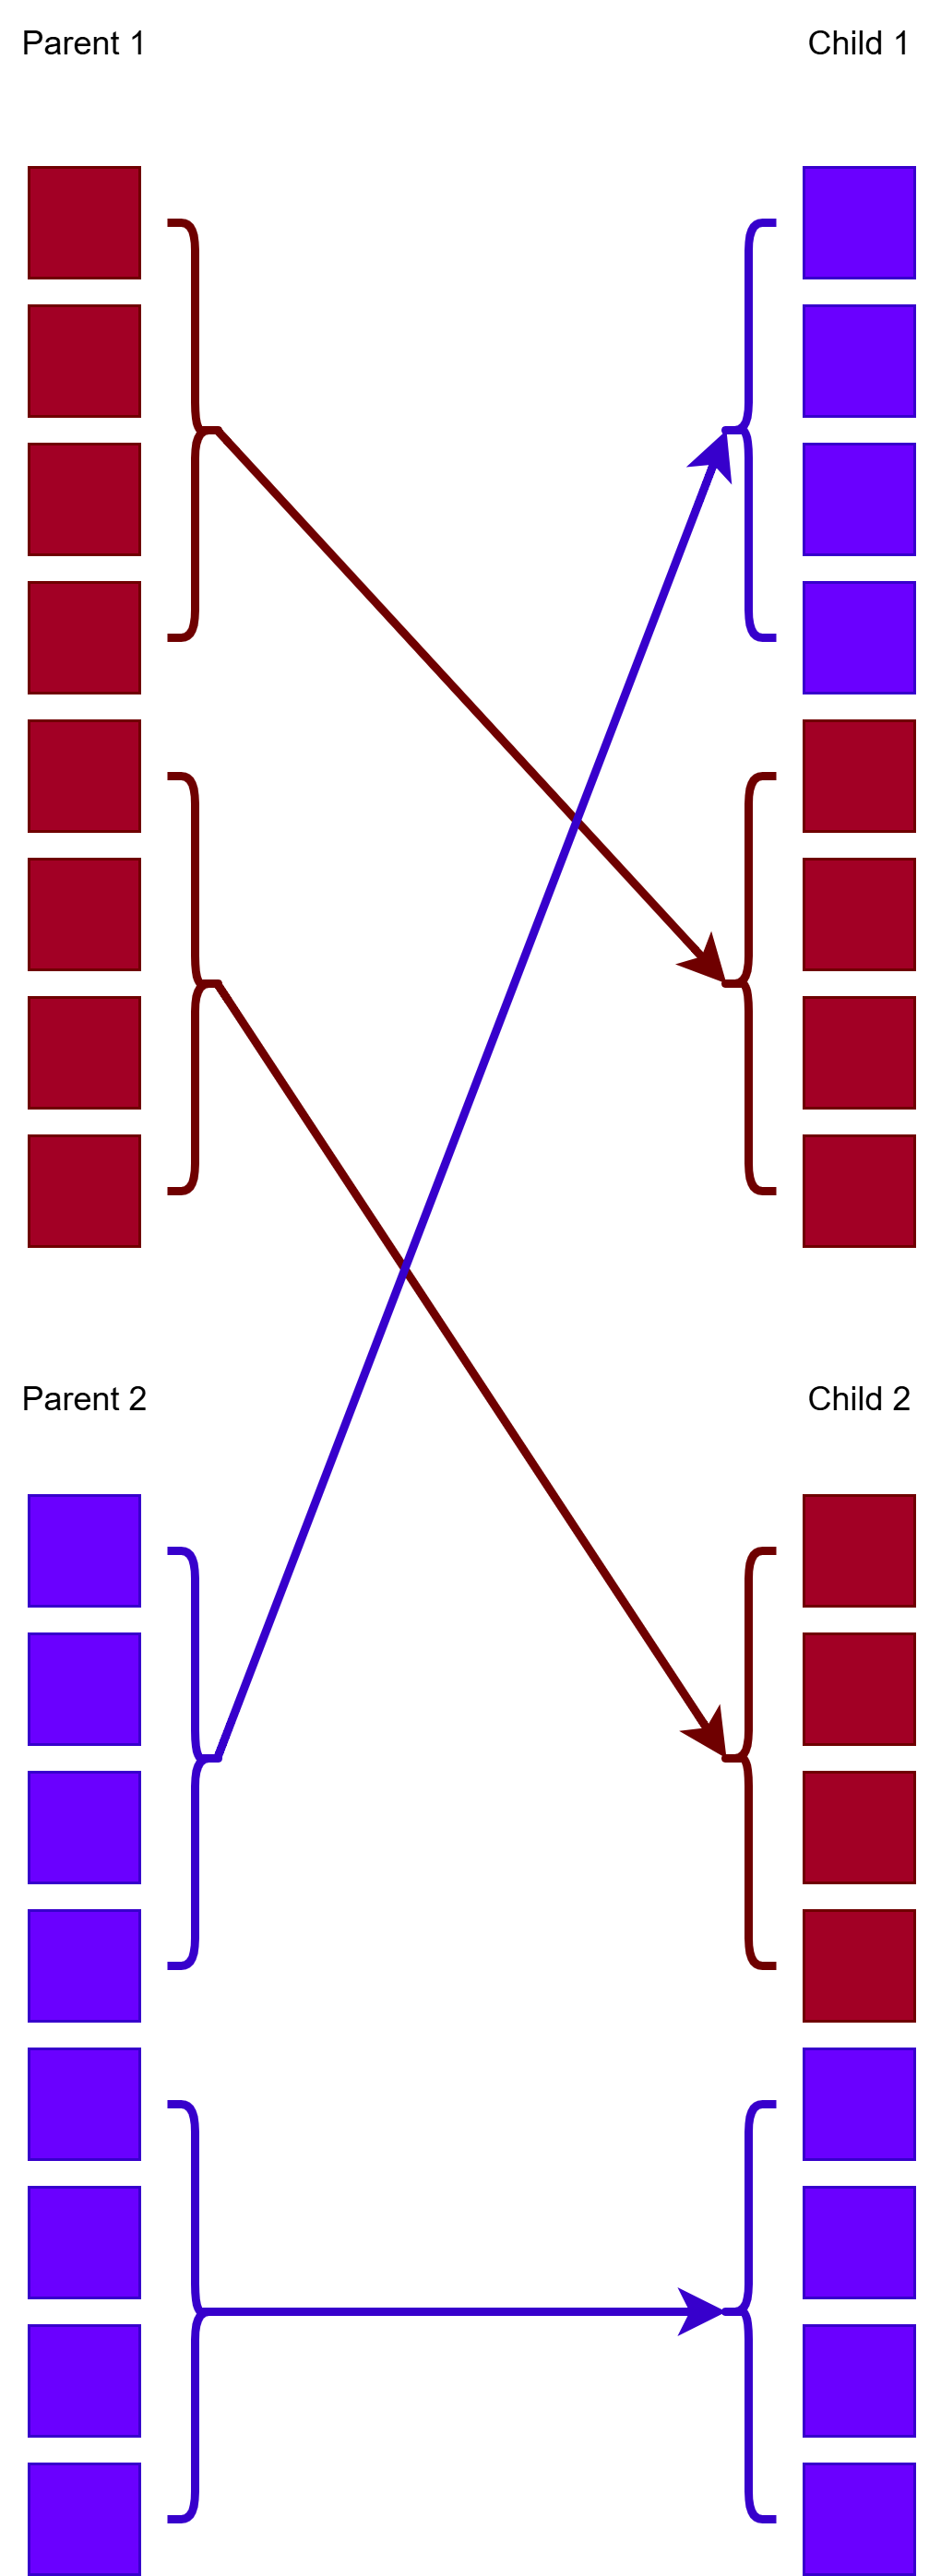
\includegraphics[scale=0.5]{cross2}
\par\end{centering}
\caption{One point crossover method, used in the Grammatical Evolution procedure.\label{fig:One-point-crossover}}
\end{figure}


\section{Results}

The code used in the experiments was code in the C++ programming language
and for the optimization methods the freely available Optimus programming
tool was incorporated \citep{optimus}. The experiments were conducted
on machine with 128GB of ram, running the Debian Linux operating system.
Each experiment was executed 30 times and the average classification
error was measured and depicted in the related tables and graphs.
Also, the 10 - fold cross validation technique was incorporated for
the validation of the experimental results. The values for the parameters
of the proposed method are depicted in Table  \ref{tab:settings}.\textbf{
}
\begin{table}[H]
\caption{The values for the parameters for the current work.\label{tab:settings}}

\centering{}%
\begin{tabular}{|c|c|c|}
\hline 
PARAMETER & MEANING & VALUE\tabularnewline
\hline 
\hline 
$N_{g}$ & Number of maximum allowed generations. & 500\tabularnewline
\hline 
$N_{c}$ & Number of chromosomes & 500\tabularnewline
\hline 
$p_{s}$ & Selection rate & 0.10\tabularnewline
\hline 
$p_{m}$ & Mutation rate & 0.05\tabularnewline
\hline 
$H$ & Number of processing nodes for neural network & 10\tabularnewline
\hline 
\end{tabular}
\end{table}
\textbf{ }

In the experimental tables the following notation is used:
\begin{enumerate}
\item The column DATASET represents the used dataset.
\item The column RBF stands for the application of an RBF neural network
\citep{rbf1,rbf2} with 10 processing nodes on the corresponding dataset.
\item The column GEN represents the application of a genetic algorithm \citep{geneticnn}
on the training process of a neural network with 10 processing nodes.
\item The column PCA stands for the application of the PCA method \citep{nnpca1,nnpca2,nnpca3}
to construct two artificial features from the original ones. Afterwards,
a neural network with 10 processing nodes trained using the BFGS method
is applied on the new datasets.
\item The column NNC stands for the application of a neural network constructed
with Grammatical Evolution \citep{nnc} on the corresponding dataset.
\item The column GENCLASS represents the usage of a method that constructs
classification rules using Grammatical Evolution \citep{genclass}.
\item The column FC2 is used to represent the application of a genetic algorithm
to train a neural network on the dataset produced by the construction
of two artificial features using the feature construction method.
\item The column FC3 is used to represent the application of a genetic algorithm
to train a neural network on the dataset produced by the construction
of three artificial features using the feature construction method.
\item The column FC4 is used to represent the application of a genetic algorithm
to train a neural network on the dataset produced by the construction
of four artificial features using the feature construction method.
\item The row AVERAGE represents the average classification error for all
datasets and the corresponding method.
\end{enumerate}
\begin{table}[H]
\caption{Experimental results for various exercises.\label{tab:exper}}

\raggedright{}{\footnotesize{}%
\begin{tabular}{|c|c|c|c|c|c|c|c|c|}
\hline 
{\footnotesize DATASET} & {\footnotesize RBF} & {\footnotesize GEN} & {\footnotesize PCA} & {\footnotesize NNC} & {\footnotesize GENCLASS} & {\footnotesize FC2} & {\footnotesize FC3} & {\footnotesize FC4}\tabularnewline
\hline 
\hline 
{\footnotesize EXERCISE\_0} & {\footnotesize 40.86\%} & {\footnotesize 39.63\%} & {\footnotesize 44.70\%} & {\footnotesize 32.57\%} & {\footnotesize 25.52\%} & {\footnotesize 11.39\%} & {\footnotesize 11.06\%} & {\footnotesize 10.35\%}\tabularnewline
\hline 
{\footnotesize EXERCISE 1} & {\footnotesize 38.65\%} & {\footnotesize 47.61\%} & {\footnotesize 47.35\%} & {\footnotesize 42.07\%} & {\footnotesize 29.98\%} & {\footnotesize 20.16\%} & {\footnotesize 16.08\%} & {\footnotesize 14.84\%}\tabularnewline
\hline 
{\footnotesize EXERCISE 2} & {\footnotesize 37.57\%} & {\footnotesize 35.33\%} & {\footnotesize 40.46\%} & {\footnotesize 35.01\%} & {\footnotesize 31.34\%} & {\footnotesize 22.50\%} & {\footnotesize 19.78\%} & {\footnotesize 22.10\%}\tabularnewline
\hline 
{\footnotesize EXERCISE 3} & {\footnotesize 41.64\%} & {\footnotesize 39.17\%} & {\footnotesize 43.46\%} & {\footnotesize 35.88\%} & {\footnotesize 29.00\%} & {\footnotesize 19.79\%} & {\footnotesize 17.39\%} & {\footnotesize 19.91\%}\tabularnewline
\hline 
\end{tabular}}{\footnotesize\par}
\end{table}
\begin{table}[H]
\caption{Precision values.\label{tab:Precision-values.}}

\raggedright{}{\footnotesize{}%
\begin{tabular}{|c|c|c|c|c|c|c|c|c|}
\hline 
{\footnotesize DATASET} & {\footnotesize RBF} & {\footnotesize GEN} & {\footnotesize PCA} & {\footnotesize NNC} & {\footnotesize GENCLASS} & {\footnotesize FC2} & {\footnotesize FC3} & {\footnotesize FC4}\tabularnewline
\hline 
\hline 
{\footnotesize EXERCISE\_0} & {\footnotesize 58.93\%} & {\footnotesize 60.30\%} & {\footnotesize 55.89\%} & {\footnotesize 67.34\%} & {\footnotesize 76.09\%} & {\footnotesize 88.51\%} & {\footnotesize 88.87\%} & {\footnotesize 89.82\%}\tabularnewline
\hline 
{\footnotesize EXERCISE 1} & {\footnotesize 61.99\%} & {\footnotesize 49.57\%} & {\footnotesize 58.12\%} & {\footnotesize 59.48\%} & {\footnotesize 71.27\%} & {\footnotesize 79.45\%} & {\footnotesize 83.66\%} & {\footnotesize 85.10\%}\tabularnewline
\hline 
{\footnotesize EXERCISE 2} & {\footnotesize 61.61\%} & {\footnotesize 72.58\%} & {\footnotesize 58.21\%} & {\footnotesize 64.62\%} & {\footnotesize 69.02\%} & {\footnotesize 77.78\%} & {\footnotesize 80.27\%} & {\footnotesize 78.01\%}\tabularnewline
\hline 
{\footnotesize EXERCISE 3} & {\footnotesize 58.33\%} & {\footnotesize 60.80\%} & {\footnotesize 56.63\%} & {\footnotesize 64.22\%} & {\footnotesize 71.52\%} & {\footnotesize 80.29\%} & {\footnotesize 82.88\%} & {\footnotesize 80.30\%}\tabularnewline
\hline 
\end{tabular}}{\footnotesize\par}
\end{table}
\begin{table}[H]
\caption{Recall values.\label{tab:Recall-values.}}

\raggedright{}{\footnotesize{}%
\begin{tabular}{|c|c|c|c|c|c|c|c|c|}
\hline 
{\footnotesize DATASET} & {\footnotesize RBF} & {\footnotesize GEN} & {\footnotesize PCA} & {\footnotesize NNC} & {\footnotesize GENCLASS} & {\footnotesize FC2} & {\footnotesize FC3} & {\footnotesize FC4}\tabularnewline
\hline 
\hline 
{\footnotesize EXERCISE\_0} & {\footnotesize 58.84\%} & {\footnotesize 60.27\%} & {\footnotesize 55.85\%} & {\footnotesize 68.92\%} & {\footnotesize 74.99\%} & {\footnotesize 88.25\%} & {\footnotesize 88.49\%} & {\footnotesize 89.27\%}\tabularnewline
\hline 
{\footnotesize EXERCISE 1} & {\footnotesize 61.90\%} & {\footnotesize 76.55\%} & {\footnotesize 60.45\%} & {\footnotesize 62.56\%} & {\footnotesize 71.11\%} & {\footnotesize 79.74\%} & {\footnotesize 83.92\%} & {\footnotesize 85.42\%}\tabularnewline
\hline 
{\footnotesize EXERCISE 2} & {\footnotesize 62.55\%} & {\footnotesize 64.58\%} & {\footnotesize 58.94\%} & {\footnotesize 65.32\%} & {\footnotesize 67.42\%} & {\footnotesize 77.06\%} & {\footnotesize 80.14\%} & {\footnotesize 78.04\%}\tabularnewline
\hline 
{\footnotesize EXERCISE 3} & {\footnotesize 58.30\%} & {\footnotesize 60.76\%} & {\footnotesize 56.67\%} & {\footnotesize 65.19\%} & {\footnotesize 71.27\%} & {\footnotesize 80.12\%} & {\footnotesize 82.65\%} & {\footnotesize 80.21\%}\tabularnewline
\hline 
\end{tabular}}{\footnotesize\par}
\end{table}


\section{Conclusions}

\vspace{6pt}


\authorcontributions{Fo}

\funding{This research has been financed by the European Union : Next Generation
EU through the Program Greece 2.0 National Recovery and Resilience
Plan , under the call RESEARCH -- CREATE -- INNOVATE, project name
“iCREW: Intelligent small craft simulator for advanced crew training
using Virtual Reality techniques\textquotedbl{} (project code:TAEDK-06195).}

\institutionalreview{Not applicable.}

\informedconsent{Not applicable.}

\conflictsofinterest{The authors declare no conflicts of interest.}

\appendix

\begin{adjustwidth}{-\extralength}{0cm}{}


\reftitle{References}
\begin{thebibliography}{99}
\bibitem{bnf1}J. W. Backus. The Syntax and Semantics of the Proposed
International Algebraic Language of the Zurich ACM-GAMM Conference.
Proceedings of the International Conference on Information Processing,
UNESCO, 1959, pp.125-132.

\bibitem{ge1}M. O’Neill, C. Ryan, Grammatical evolution, IEEE Trans.
Evol. Comput. \textbf{5,}pp. 349--358, 2001.

\bibitem{nn1}C. Bishop, Neural Networks for Pattern Recognition,
Oxford University Press, 1995.

\bibitem{nn2}G. Cybenko, Approximation by superpositions of a sigmoidal
function, Mathematics of Control Signals and Systems \textbf{2}, pp.
303-314, 1989.

\bibitem{fc1}Dimitris Gavrilis, Ioannis G. Tsoulos, Evangelos Dermatas,
Selecting and constructing features using grammatical evolution, Pattern
Recognition Letters \textbf{29},pp. 1358-1365, 2008. 

\bibitem{fc2}Dimitris Gavrilis, Ioannis G. Tsoulos, Evangelos Dermatas,
Neural Recognition and Genetic Features Selection for Robust Detection
of E-Mail Spam, Advances in Artificial Intelligence Volume 3955 of
the series Lecture Notes in Computer Science pp 498-501, 2006.

\bibitem{fc3}George Georgoulas, Dimitris Gavrilis, Ioannis G. Tsoulos,
Chrysostomos Stylios, João Bernardes, Peter P. Groumpos, Novel approach
for fetal heart rate classification introducing grammatical evolution,
Biomedical Signal Processing and Control \textbf{2},pp. 69-79, 2007 

\bibitem{fc4}Otis Smart, Ioannis G. Tsoulos, Dimitris Gavrilis, George
Georgoulas, Grammatical evolution for features of epileptic oscillations
in clinical intracranial electroencephalograms, Expert Systems with
Applications \textbf{38}, pp. 9991-9999, 2011 

\bibitem{fc5}A. T. Tzallas, I. Tsoulos, M. G. Tsipouras, N. Giannakeas,
I. Androulidakis and E. Zaitseva, Classification of EEG signals using
feature creation produced by grammatical evolution, In: 24th Telecommunications
Forum (TELFOR), pp. 1-4, 2016.

\bibitem[(2025)]{optimus}I.G. Tsoulos, V. Charilogis, G. Kyrou, V.N.
Stavrou, A. Tzallas, Journal of Open Source Software \textbf{10},
7584, 2025.

\bibitem[(1991)]{rbf1}J. Park and I. W. Sandberg, Universal Approximation
Using Radial-Basis-Function Networks, Neural Computation \textbf{3},
pp. 246-257, 1991.

\bibitem{rbf2}G.A. Montazer, D. Giveki, M. Karami, H. Rastegar, Radial
basis function neural networks: A review. Comput. Rev. J \textbf{1},
pp. 52-74, 2018.

\bibitem[(1989)]{geneticnn}Reynolds, J., Rezgui, Y., Kwan, A., \&
Piriou, S. (2018). A zone-level, building energy optimisation combining
an artificial neural network, a genetic algorithm, and model predictive
control. Energy, 151, 729-739.

\bibitem{nnpca1}Burcu Erkmen, Tülay Yıldırım, Improving classification
performance of sonar targets by applying general regression neural
network with PCA, Expert Systems with Applications \textbf{35}, pp.
472-475, 2008.

\bibitem{nnpca2}Jing Zhou, Aihuang Guo, Branko Celler, Steven Su,
Fault detection and identification spanning multiple processes by
integrating PCA with neural network, Applied Soft Computing \textbf{14},
pp. 4-11, 2014.

\bibitem{nnpca3}Ravi Kumar G., Nagamani K., Anjan Babu G., A Framework
of Dimensionality Reduction Utilizing PCA for Neural Network Prediction.
In: Borah S., Emilia Balas V., Polkowski Z. (eds) Advances in Data
Science and Management. Lecture Notes on Data Engineering and Communications
Technologies, vol 37. Springer, Singapore. 2020.

\bibitem{nnc}I.G. Tsoulos, D. Gavrilis, E. Glavas, Neural network
construction and training using grammatical evolution, Neurocomputing
\textbf{72}, pp. 269-277, 2008.

\bibitem[(1989)]{genclass}Nikolaos Anastasopoulos and Ioannis G.
Tsoulos and Alexandros Tzallas, GenClass: A parallel tool for data
classification based on Grammatical Evolution, SoftwareX, 16, 100830,
2021.

\end{thebibliography}
%%%%%%%%%%%%%%%%%%%%%%%%%%%%%%%%%%%%%%%%%%
%% for journal Sci
%\reviewreports{\\
%Reviewer 1 comments and authors' response\\
%Reviewer 2 comments and authors' response\\
%Reviewer 3 comments and authors' response
%}
%%%%%%%%%%%%%%%%%%%%%%%%%%%%%%%%%%%%%%%%%%

\PublishersNote{}

\end{adjustwidth}{}
\end{document}
